%===============================================================
% main.tex — File chính của báo cáo/đồ án BKU
% Thay các giá trị trong phần CẤU HÌNH bên dưới trước khi dùng.
%===============================================================
\documentclass[12pt, a4paper]{bkureport}

\usepackage{amsmath}
\usepackage{amssymb}

%---------------------------------------------------------------
% CẤU HÌNH — chỉnh tại đây
%---------------------------------------------------------------
\renewcommand{\BKUsubject}{BÀI TẬP LỚN MÔN EE2015}
\newcommand{\TenDeTai}{WEBFFT — ỨNG DỤNG WEB MÔ PHỎNG DFT/FFT VÀ XỬ LÝ ÂM THANH THỜI GIAN THỰC}
\newcommand{\TenGVHD}{Tên Giảng Viên hướng dẫn}
\newcommand{\TenSVTH}{Họ và Tên Sinh Viên}
\newcommand{\MSSV}{Mã số sinh viên}
\newcommand{\NgayBaoCao}{tháng 5 năm 2026}
%---------------------------------------------------------------

\begin{document}

	%----- SỐ TRANG LA MÃ (bìa, lời cảm ơn, tóm tắt, mục lục) -----
	\pagenumbering{Roman}

	%===============================================================
% bia.tex — Trang bìa
% Các biến \TenDeTai, \TenGVHD, \TenSVTH, \MSSV, \NgayBaoCao
% được khai báo trong main.tex
%===============================================================
\setlength{\parindent}{0pt}

\begin{titlepage}

	% --- Khung trang bìa ---
	\begin{tikzpicture}[remember picture, overlay]
	\draw [line width=1pt]
	($ (current page.north west) + (3.0cm,-2.0cm) $)
	rectangle
	($ (current page.south east) + (-2.0cm,3.0cm) $);
	\draw [line width=3pt]
	($ (current page.north west) + (2.85cm,-1.85cm) $)
	rectangle
	($ (current page.south east) + (-1.85cm,2.85cm) $);
	\end{tikzpicture}

	% --- Thông tin trường ---
	\begin{center}
		\vspace{7pt}
		\textbf{
			ĐẠI HỌC QUỐC GIA THÀNH PHỐ HỒ CHÍ MINH\\
			TRƯỜNG ĐẠI HỌC BÁCH KHOA THÀNH PHỐ HỒ CHÍ MINH\\
		}
		\vspace{7pt}
		\textbf{KHOA ĐIỆN - ĐIỆN TỬ}\\
		\textbf{BỘ MÔN VIỄN THÔNG}\\
		\textbf{--------------------  *  ---------------------}\\[1cm]
	\end{center}

	\begin{center}
		
\includegraphics[width=0.25\textwidth]{images/logo-bku.png}\\[1.5cm]
		{\large \BKUsubject}\\[2cm]
		{\LARGE \textbf{\parbox[c][3cm]{14cm}{\centering \TenDeTai}}}\\[3.2cm]
	\end{center}

	% --- Thông tin sinh viên ---
	\hspace{5cm}\parbox[t]{10cm}{
		\textbf{GVHD: \TenGVHD}\\[3pt]
		\textbf{SVTH: \TenSVTH}\\[3pt]
		\textbf{MSSV: \MSSV}
	}
	\vfill

	\begin{center}
		\textbf{Thành phố Hồ Chí Minh, \NgayBaoCao}
	\end{center}

\end{titlepage}

	\pagestyle{plain}
	%===============================================================
% loicamon.tex — Lời cảm ơn
%===============================================================
\pagestyle{empty}
\begin{center}
	{\Large\textbf{\textcolor{red}{LỜI CẢM ƠN}}}
\end{center}

\vspace{1cm}

\hspace*{2em} Em xin gửi lời cảm ơn chân thành đến thầy \TenGVHD{} đã nhiệt tình giúp đỡ và chỉ dẫn em trong suốt quá trình thực hiện đề tài. Nhờ sự hướng dẫn tận tình và những góp ý quý báu của thầy mà em đã hoàn thành tốt được đồ án. Em xin gửi lời cảm ơn đến quý thầy cô đã dạy dỗ và cung cấp kiến thức có liên quan để em có thể thực hiện được đề tài này một cách hiệu quả. Mặc dù vậy, trong quá trình thực hiện đề tài khó tránh khỏi sai sót, mong thầy cô đánh giá và nhận xét để em có thể hoàn thành những đề tài sau được tốt hơn. Em xin chân thành cảm ơn!

\vspace{6cm}

\hfill
\begin{minipage}{0.5\textwidth}
	\begin{center}
		TP. Hồ Chí Minh, \NgayBaoCao\\[0.3cm]
		\textbf{Sinh viên}\\[1.2cm]
		\vspace{3cm}
		\TenSVTH
	\end{center}
\end{minipage}

	%===============================================================
% tomtat.tex — Tóm tắt đề tài
%===============================================================
\begin{center}
	\textbf{{\Large\textcolor{black}{TÓM TẮT ĐỀ TÀI}}}
\end{center}

\vspace{1cm}

\hspace*{2cm}
Đề tài xây dựng \textit{WebFFT} --- một ứng dụng web đơn trang (SPA) chạy hoàn toàn trên trình duyệt, không máy chủ xử lý âm thanh: vừa phục vụ học tập nguyên lý biến đổi Fourier rời rạc (DFT) và thuật toán FFT (sơ đồ butterfly tương tác), vừa minh họa các bài toán xử lý tín hiệu âm thanh thời gian thực gồm phân tích phổ và spectrogram, giải mã đa tần DTMF, khử nhiễu kiểu trừ phổ trong AudioWorklet, và ước lượng cao độ bằng thuật toán YIN cho bộ chỉnh âm nhạc cụ.

Phương pháp thực hiện dựa trên JavaScript (ES modules), Web Audio API (\texttt{AudioContext}, \texttt{AnalyserNode}, \texttt{OscillatorNode}), AudioWorklet cho luồng audio độ trễ thấp, và các mô-đun DSP tự cài đặt (DFT, FFT radix-2, STFT, số phức) trong thư mục \verb|src/dsp/|. Giao diện gồm năm chế độ độc lập theo tab, điều hướng bằng URL hash; ứng dụng có thể triển khai tĩnh và hỗ trợ PWA (manifest, service worker). Toàn bộ dữ liệu âm thanh được xử lý cục bộ trên máy người dùng.

Kết quả đạt được là một công cụ trực quan, đa nền tảng, có kiểm thử đơn vị (\texttt{npm test}) cho các thành phần DSP và giải mã chọn lọc; báo cáo trình bày cơ sở lý thuyết, kiến trúc phần mềm, chi tiết triển khai thuật toán và đánh giá chức năng cùng hướng phát triển tiếp theo.


	%----- MỤC LỤC -----
	\pagestyle{empty}
	\tableofcontents
	\clearpage

	%----- DANH MỤC ẢNH -----
	\pagestyle{empty}
	\listoffigures
	\clearpage

	%----- DANH MỤC BẢNG -----
	\pagestyle{empty}
	\listoftables
	\clearpage

	%----- DANH MỤC CHỮ VIẾT TẮT -----
	\chapter*{{\Large\begin{center}DANH MỤC CHỮ VIẾT TẮT\end{center}}}
	%===============================================================
% viettat.tex — Danh mục chữ viết tắt
%===============================================================
\begin{table}[h!]
	\centering
	\begin{tabular}{ll}
		API     & Application Programming Interface \\
		COLA    & Constant Overlap-Add (điều kiện tái tạo khi STFT/IFFT chồng khung) \\
		DFT     & Discrete Fourier Transform \\
		DSP     & Digital Signal Processing \\
		DTMF    & Dual-Tone Multi-Frequency \\
		FFT     & Fast Fourier Transform \\
		IDFT    & Inverse Discrete Fourier Transform \\
		IFFT    & Inverse Fast Fourier Transform \\
		ITU     & International Telecommunication Union \\
		PCM     & Pulse Code Modulation \\
		PWA     & Progressive Web App \\
		SPA     & Single Page Application \\
		STFT    & Short-Time Fourier Transform \\
		SW      & Service Worker \\
		WASM    & WebAssembly \\
	\end{tabular}
\end{table}

	\pagestyle{empty}
	\clearpage

	%----- CÁC CHƯƠNG NỘI DUNG -----
	\pagenumbering{arabic}
	\pagestyle{fancy}

	% Trang đầu chương cũng có header/footer
	\fancypagestyle{plain}{
		\fancyhf{}
		\fancyhead[L]{\BKUsubject}
		\fancyhead[R]{\leftmark}
		\fancyfoot[C]{\thepage}
		\renewcommand{\headrulewidth}{1pt}
		\renewcommand{\footrulewidth}{1pt}
	}

	%===============================================================
% chap1.tex — Chương 1: Giới thiệu
%===============================================================
\pagestyle{fancy}
\chapter{GIỚI THIỆU}

\section{Tổng quan đề tài}
Biến đổi Fourier rời rạc (DFT) và biến đổi Fourier nhanh (FFT) là nền tảng của nhiều hệ thống xử lý tín hiệu số: phân tích phổ, lọc dựa trên miền tần số, nén và truyền thông. Việc chỉ đọc lý thuyết trên giấy thường khó hình dung cấu trúc tính toán và đánh đổi độ phân giải thời gian--tần số trong xử lý âm thanh thực tế.

Đề tài xây dựng ứng dụng \textbf{WebFFT} --- một SPA chạy trên trình duyệt hiện đại, cho phép người dùng (1) mô phỏng DFT/FFT trên dãy nhỏ và quan sát sơ đồ butterfly; (2) phân tích phổ và spectrogram từ micro thời gian thực; (3) phát và nhận dạng tín hiệu DTMF; (4) demo khử nhiễu kiểu trừ phổ trong AudioWorklet; (5) ước lượng cao độ nhạc cụ bằng thuật toán YIN. Toàn bộ xử lý âm thanh thực hiện \textit{cục bộ} trên máy khách, không gửi buffer lên máy chủ \cite{repoWebFFT}.

\section{Nhiệm vụ đề tài}

\noindent\textbf{Nội dung 1: Mô phỏng DFT/FFT và visualization học tập.}\\
\vspace{-0.6cm}
\begin{itemize}\itemsep0pt \parskip0pt \parsep0pt
	\item \textbf{Mục tiêu:} Giúp người học nhập tín hiệu rời rạc (thực hoặc phức), so sánh kết quả DFT ngây thơ và FFT radix-2, quan sát cấu trúc butterfly.
	\item \textbf{Ý tưởng thực hiện:} Module \verb|src/dsp/dft.js|, \verb|src/dsp/fft.js|, \verb|src/dsp/butterflyData.js|; giao diện \verb|src/ui/dftSimulator.js| và SVG tương tác \verb|src/visualization/butterflySvg.js|.
\end{itemize}
\vspace{-0.2cm}

\noindent\textbf{Nội dung 2: Phân tích phổ và STFT thời gian thực.}\\
\vspace{-0.6cm}
\begin{itemize}\itemsep0pt \parskip0pt \parsep0pt
	\item \textbf{Mục tiêu:} Hiển thị phổ biên độ và spectrogram từ micro; so sánh cửa sổ và có thể đối chiếu FFT nội bộ với pipeline trình duyệt.
	\item \textbf{Ý tưởng thực hiện:} \verb|AnalyserNode|, \verb|src/dsp/stft.js|, \verb|src/ui/spectrumAnalyzer.js|, \verb|src/visualization/spectrumCanvas.js|.
\end{itemize}
\vspace{-0.2cm}

\noindent\textbf{Nội dung 3: Giải mã DTMF.}\\
\vspace{-0.6cm}
\begin{itemize}\itemsep0pt \parskip0pt \parsep0pt
	\item \textbf{Mục tiêu:} Phát hai tone chuẩn hoặc thu qua micro và nhận dạng phím (hàng/cột).
	\item \textbf{Ý tưởng thực hiện:} FFT sau cửa sổ Hann, tìm hai đỉnh trong dải tần ITU \cite{ituQ23}; \verb|src/ui/dtmfDecoder.js|.
\end{itemize}
\vspace{-0.2cm}

\noindent\textbf{Nội dung 4: Khử nhiễu trừ phổ.}\\
\vspace{-0.6cm}
\begin{itemize}\itemsep0pt \parskip0pt \parsep0pt
	\item \textbf{Mục tiêu:} Cho phép học mẫu nhiễu và làm sạch giọng nói theo khung STFT trên luồng audio độ trễ thấp.
	\item \textbf{Ý tưởng thực hiện:} STFT $N{=}1024$, hop 50\%, cửa sqrt-Hann thỏa COLA; spectral subtraction trong \verb|src/audioWorklet/noiseReducer.js|.
\end{itemize}
\vspace{-0.2cm}

\noindent\textbf{Nội dung 5: Bộ chỉnh âm (YIN).}\\
\vspace{-0.6cm}
\begin{itemize}\itemsep0pt \parskip0pt \parsep0pt
	\item \textbf{Mục tiêu:} Ước lượng tần số cơ bản và sai số cent so với nốt nhạc gần nhất.
	\item \textbf{Ý tưởng thực hiện:} \verb|src/dsp/yin.js|, hiển thị \verb|src/visualization/tunerDisplay.js|.
\end{itemize}
\vspace{-0.2cm}

\section{Bố cục đề tài}
Báo cáo gồm năm chương nội dung và phần kết luận. \textbf{Chương 2} trình bày cơ sở lý thuyết về lấy mẫu, DFT/FFT, STFT, DTMF, trừ phổ, YIN và Web Audio. \textbf{Chương 3} mô tả kiến trúc SPA, phân tầng mã nguồn và luồng dữ liệu âm thanh. \textbf{Chương 4} chi tiết thiết kế và triển khai từng chế độ cùng kiểm thử. \textbf{Chương 5} trình bày kết quả chạy thử, đánh giá định tính và gợi ý đánh giá định lượng. Phần \textbf{Kết luận} tóm tắt đóng góp và hướng phát triển; danh mục tài liệu tham khảo đặt cuối báo cáo.

	%===============================================================
% chap2.tex — Chương 2: Cơ sở lý thuyết
%===============================================================
\pagestyle{fancy}
\chapter{CƠ SỞ LÝ THUYẾT}

\section{Lấy mẫu và tín hiệu rời rạc}
Tín hiệu âm thanh liên tục $x_a(t)$ được lấy mẫu với chu kỳ $T_s$, tạo dãy $x[n]=x_a(nT_s)$, tần số lấy mẫu $f_s=1/T_s$. Định lý lấy mẫu (Nyquist--Shannon) yêu cầu băng thông có giới hạn sao cho $f_s > 2 f_{\max}$ để tránh chồng phổ (aliasing). Trong WebFFT, âm thanh từ micro hoặc \texttt{AudioContext} đã được card âm thanh / trình duyệt lượng tử hoá ở $f_s$ thông dụng (thường 44,1 kHz hoặc 48 kHz); người dùng chọn kích thước FFT (\texttt{fftSize}) ảnh hưởng độ phân giải tần $\Delta f = f_s/N$ và độ trễ quan sát \cite{oppenheim}.

\section{Biến đổi Fourier rời rạc (DFT) và thuật toán FFT}
Với dãy phức độ dài $N$, DFT định nghĩa
\begin{equation}
	X[k]=\sum_{n=0}^{N-1} x[n]\, e^{-j 2\pi kn/N}, \qquad k=0,\ldots,N-1.
\end{equation}
IDFT khôi phục $x[n]$ từ $X[k]$ với hệ số chuẩn hoá $1/N$. DFT trực tiếp có độ phức tạp $O(N^2)$, thích hợp cho mô phỏng giáo dục trên $N$ nhỏ trong Simulator.

Thuật toán FFT radix-2 Cooley--Tukey tận dụng phân rã đệ quy và tính chất tuần hoàn của hệ số quay pha (twiddle), giảm độ phức tạp xuống $O(N\log N)$ khi $N$ là lũy thừa 2 \cite{cooleyJW}. Cấu trúc tính toán biểu diễn bằng các ``bướm'' hai đầu vào hai đầu ra (butterfly). Trong mã nguồn, FFT và IFFT phục vụ khử nhiễu và các chức năng phân tích nội bộ được triển khai trong \verb|src/dsp/fft.js| và tái sử dụng trong AudioWorklet.

\section{STFT, spectrogram và cửa sổ thời gian}
Để phân tích tín hiệu không dừng, ta chia khung độ dài $N$, nhân cửa sổ $w[n]$ giảm rò mép (spectral leakage), rồi DFT từng khung:
\begin{equation}
	X[m,k]=\sum_{n=0}^{N-1} x[n+mH]\, w[n]\, e^{-j 2\pi kn/N},
\end{equation}
với $H$ là bước nhảy (hop). Spectrogram là $|X[m,k]|$ hoặc biên độ log theo thời gian $m$. Độ phân giải tần và thời gian đánh đổi nhau khi thay $N$, $H$ và kiểu cửa (Hann, Hamming, Blackman---hệ số được dùng trong Analyzer và trong các chỗ cần so sánh với pipeline DSP).

\section{Đa tần DTMF và phát hiện hai thành phần tần số}
DTMF kết hợp một tần thấp (nhóm hàng) và một tần cao (nhóm cột) trong các giá trị chuẩn hoá quốc tế \cite{ituQ23}. Nguyên lý nhận dạng trong miền tần: sau cửa sổ và FFT, tìm hai đỉnh biên độ rõ trong hai dải hàng và cột; ghép cặp suy ra ký tự phím. Phương pháp đơn giản nhưng đủ minh hoạ liên hệ giữa phân tích phổ và ra quyết định.

\section{Khử nhiễu kiểu trừ phổ (spectral subtraction)}
Giả thuyết thống kê gọn thường dùng trong giảng dạy: phổ quan sát $Y[k]$ gần bằng tín hiệu sạch $S[k]$ cộng nhiễu $N[k]$ theo năng lượng
\begin{equation}
	|Y[k]|^2 \approx |S[k]|^2 + |N[k]|^2 .
\end{equation}
Ước lượng $|N[k]|$ từ khung chỉ có nhiễu (noise prototype), sau đó suy ra biên độ sạch $\hat{S}[k]$ bằng trừ (và giới hạn sàn nhiễu để tránh artefact âm ``musical noise'' \cite{oppenheim}). Triển khai trong đề tài dùng STFT khung cố định và tái tạo miền thời gian qua IFFT chồng khung (COLA với sqrt-Hann), chi tiết lập trình xem \verb|noiseReducer.js|.

\section{Ước lượng cao độ và thuật toán YIN}
YIN ước lượng chu kỳ cơ bản $\tau$ (đơn vị mẫu) bằng hàm sai khác bình phương và phiên bản chuẩn hoá trung bình lũy kế (CMND)\footnote{Cumulative Mean Normalized Difference --- trong mã gọi là CMD theo biến \texttt{cmd}.}, sau đó tìm cực tiểu dưới ngưỡng tin cậy; nội suy parabol quanh cực tiểu cải thiện độ phân giải tần số \cite{cheveigne2002}. Tần số $f_0 = f_s/\tau$. Sai số cao độ so với nốt nhạc chuẩn thường biểu diễn bằng cent: một octave $=1200$ cent.

\section{Web Audio API và luồng xử lý thời gian thực}
\texttt{AudioContext} quản lý đồ thị nút âm thanh: nguồn (\texttt{MediaStreamAudioSourceNode}, \texttt{OscillatorNode}), xử lý (\texttt{GainNode}), và phân tích (\texttt{AnalyserNode}). Luồng render âm thanh chạy trên luồng riêng độ trễ thấp; \texttt{AudioWorklet} cho phép chèn xử lý mẫu theo mẫu hoặc khối PCM đồng bộ với đồng hồ âm thanh, phù hợp FFT/IFFT khử nhiễu \cite{mdnWorklet}. \texttt{AnalyserNode.getFloatTimeDomainData} cung cấp PCM cho tuner và có thể kết hợp với pipeline FFT của trình duyệt để vẽ phổ mượt \cite{mdnAudio}.

	%===============================================================
% chap3.tex — Chương 3: Thiết kế kiến trúc hệ thống
%===============================================================
\pagestyle{fancy}
\chapter{THIẾT KẾ KIẾN TRÚC HỆ THỐNG}

\section{Tổng quan và kiểu hệ thống}
WebFFT là SPA không máy chủ ứng dụng: máy chủ (nếu có) chỉ phục vụ file tĩnh (\texttt{index.html}, \texttt{src/*.js}, CSS, asset). Mọi DSP và truy cập micro diễn ra trong trình duyệt người dùng. Ứng dụng có thể ``cài'' như PWA nhờ \texttt{manifest.json} và service worker \texttt{sw.js} để cache ngoại tuyến một phần tài nguyên.

\section{Phân tầng phần mềm}
\begin{itemize}\itemsep2pt
	\item \textbf{Tầng DSP thuần} (\verb|src/dsp/|): số phức, DFT, FFT/IFFT, STFT, YIN, dữ liệu butterfly --- không phụ thuộc DOM hay Web Audio, tiện kiểm thử Node.
	\item \textbf{Tầng âm thanh} (\verb|src/audioEngine.js|, \verb|src/audioWorklet/|): khởi tạo \texttt{AudioContext}, chia sẻ luồng micro, resume sau autoplay policy; worklet \texttt{pcmCapture}, \texttt{noiseReducer}.
	\item \textbf{Tầng UI theo chế độ} (\verb|src/ui/|): mỗi tab một factory (\texttt{createDftSimulatorMode}, \ldots); \verb|uiManager.js| điều phối hiển thị và vòng đời mode.
	\item \textbf{Tầng visualization} (\verb|src/visualization/|): Canvas phổ/spectrogram, SVG butterfly, vẽ tuner.
\end{itemize}

\section{Điều phối ứng dụng và điều hướng}
File \verb|src/app.js| khai báo thứ tự tab \texttt{simulator}, \texttt{analyzer}, \texttt{dtmf}, \texttt{noise}, \texttt{tuner}; đồng bộ với nút tab trong HTML và URL hash (\texttt{\#simulator}, \ldots). Khi đổi tab:
\begin{itemize}\itemsep2pt
	\item Tab không cần micro realtime (Simulator) có thể giải phóng micro và phát sự kiện \texttt{webfft:stop-audio}.
	\item Tab realtime hiển thị nhóm nút điều khiển âm thanh và ẩn/hiện theo \texttt{isRealtimeAudio}.
\end{itemize}

\section{Luồng dữ liệu âm thanh}
Hình \ref{fig:arch-webfft} minh hoạ luồng tổng quát. Micro được mở qua \texttt{getUserMedia}, đưa vào \texttt{AudioContext}. Analyzer và DTMF nhánh chính dùng \texttt{AnalyserNode} để lấy miền thời gian hoặc phổ nội bộ trình duyệt. Khử nhiễu ghép \texttt{AudioWorkletNode} với mã trong \verb|noiseReducer.js|. Simulator không bắt buộc micro; Tuner đọc PCM và gọi YIN trên main thread (buffer từ analyser hoặc capture --- xem \verb|tuner.js|).

\begin{figure}[htbp]
	\centering
	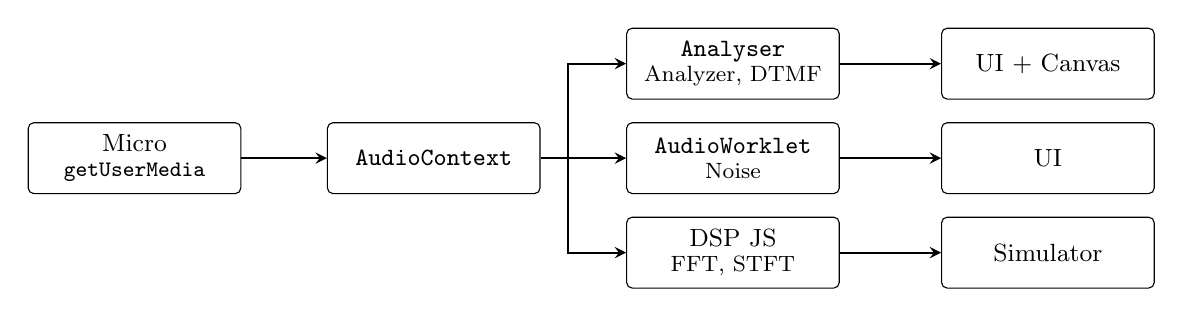
\begin{tikzpicture}[
		font=\small,
		box/.style={rectangle, draw, rounded corners=2pt, minimum width=2.7cm, minimum height=0.9cm, align=center},
		arr/.style={->, >=stealth, thick}
	]
		\node[box] (mic) at (0,0) {Micro\\[-2pt]\footnotesize\texttt{getUserMedia}};
		\node[box] (ctx) at (3.8,0) {\texttt{AudioContext}};
		\node[box] (an) at (7.6,1.2) {\texttt{Analyser}\\[-2pt]\footnotesize Analyzer, DTMF};
		\node[box] (wk) at (7.6,0) {\texttt{AudioWorklet}\\[-2pt]\footnotesize Noise};
		\node[box] (dsp) at (7.6,-1.2) {DSP JS\\[-2pt]\footnotesize FFT, STFT};
		\node[box] (ui1) at (11.6,1.2) {UI + Canvas};
		\node[box] (ui2) at (11.6,0) {UI};
		\node[box] (sim) at (11.6,-1.2) {Simulator};
		\draw[arr] (mic) -- (ctx);
		\draw[arr] (ctx.east) -- ++(0.35,0) |- (an.west);
		\draw[arr] (ctx) -- (wk.west);
		\draw[arr] (ctx.east) -- ++(0.35,0) |- (dsp.west);
		\draw[arr] (an) -- (ui1);
		\draw[arr] (wk) -- (ui2);
		\draw[arr] (dsp) -- (sim);
	\end{tikzpicture}
	\caption{Sơ đồ khối luồng dữ liệu WebFFT (đơn giản hoá).}
	\label{fig:arch-webfft}
\end{figure}

\section{Triển khai và ràng buộc môi trường}
Trình duyệt chỉ cho phép micro và \texttt{AudioContext} chạy trong ngữ cảnh bảo mật (\texttt{https} hoặc \texttt{localhost}). iOS/Safari thường yêu cầu cử chỉ người dùng trước khi phát/resume audio; tab nền có thể đình chỉ context tiết kiệm pin. Ứng dụng hiện xử lý \textbf{mono} để đơn giản hoá pipeline và khớp worklet.

	%===============================================================
% chap4.tex — Chương 4: Thiết kế và triển khai giải thuật phần mềm
%===============================================================
\pagestyle{fancy}
\chapter{THIẾT KẾ VÀ TRIỂN KHAI GIẢI THUẬT PHẦN MỀM}

\section{Mô-đun DSP dùng chung}
\texttt{complex.js} định nghĩa phép toán số phức phục vụ DFT phức trong Simulator. \texttt{dft.js} triển khai DFT/IDFT độ phức tạp $O(N^2)$ cho giáo trình. \texttt{fft.js} xuất FFT radix-2 và IFFT cùng quy ước pha $\mathrm{e}^{-2\pi ijk/N}$, được \verb|noiseReducer.js| nhúng lại (phiên bản Float32 trong worklet). \texttt{stft.js} gói cửa sổ và FFT nội bộ cho Analyzer khi cần đối chiếu với \texttt{AnalyserNode}. \texttt{dsp.js} tái xuất API gọn cho các module UI.

\section{DFT Simulator và sơ đồ butterfly}
Người dùng nhập dãy độ dài $N$ (thực hoặc phức). Simulator gọi DFT từng bước hoặc FFT tùy chế độ so sánh; \texttt{butterflyData.js} sinh cấu trúc tầng FFT để \texttt{butterflySvg.js} (D3.js) vẽ SVG tương tác. KaTeX trong trang hiển thị công thức nhất quán với báo cáo.

\section{Spectrum Analyzer}
Luồng micro vào \texttt{AnalyserNode}; UI lấy miền thời gian hoặc phổ FFT theo API trình duyệt, đồng thời có nhánh gọi STFT trong \texttt{spectrumAnalyzer.js} để nhân cửa sổ Hann/Hamming/Blackman và FFT trong JS, hiển thị chồng lên hoặc đối chiếu như mô tả README dự án. \texttt{spectrumCanvas.js} vẽ thanh phổ và waterfall spectrogram trên Canvas.

\section{Bộ giải mã DTMF}
Hai \texttt{OscillatorNode} tạo tone chuẩn khi chọn nguồn nội bộ; khi chọn micro, chỉ phân tích luồng thu được để tránh phản hồi. Khung PCM qua cửa sổ Hann rồi FFT (\texttt{dsp}); tìm cực đại cục bộ trong các dải hàng/cột ITU \cite{ituQ23}, ánh xạ sang phím.

\section{Khử nhiễu thời gian thực}
\texttt{pcmCapture.js} và UI \texttt{noiseReduction.js} cho phép ghi prototype nhiễu (vector biên độ phổ trung bình). Worklet \texttt{noiseReducer.js} chia khung $N=1024$, hop $512$, sqrt-Hann thỏa COLA; vòng lặp spectral subtraction, IFFT, overlap-add, giới hạn biên độ đầu ra.

\section{Instrument Tuner (YIN)}
PCM mono đưa vào \texttt{yinDetectPitchHz} (\texttt{yin.js}): hàm sai khác, CMD, ngưỡng 0{,}15, nội suy parabol quanh cực tiểu. \texttt{tunerDisplay.js} ánh xạ Hz sang nốt và độ lệch cent.

\section{Kiểm thử tự động}
Bộ \verb|tests/| (\texttt{node --test}): \texttt{dsp.test.js}, \texttt{butterflyData.test.js}, \texttt{dtmf.test.js}, \texttt{yin.test.js}. Lệnh \texttt{npm test} giúp hồi quy khi sửa FFT hoặc nhận dạng.

\begin{table}[htbp]
	\centering
	\caption{Bản đồ chức năng chính tới file mã nguồn}
	\label{tab:module-map}
	\begin{tabular}{@{}p{4.2cm}p{9cm}@{}}
		\toprule
		\textbf{Chức năng} & \textbf{File / thư mục chính} \\
		\midrule
		Simulator DFT/FFT & \texttt{dftSimulator.js}, \texttt{dft.js}, \texttt{fft.js}, \texttt{butterflyData.js}, \texttt{butterflySvg.js} \\
		Analyzer & \texttt{spectrumAnalyzer.js}, \texttt{spectrumCanvas.js}, \texttt{stft.js} \\
		DTMF & \texttt{dtmfDecoder.js} \\
		Noise reduction & \texttt{noiseReduction.js}, \texttt{noiseReducer.js}, \texttt{pcmCapture.js} \\
		Tuner & \texttt{tuner.js}, \texttt{yin.js}, \texttt{tunerDisplay.js} \\
		\bottomrule
	\end{tabular}
\end{table}

	%===============================================================
% chap5.tex — Chương 5: Kết quả thực hiện và đánh giá
%===============================================================
\pagestyle{fancy}
\chapter{KẾT QUẢ THỰC HIỆN VÀ ĐÁNH GIÁ}

\section{Môi trường thử nghiệm}
Đề tài chạy như ứng dụng web tĩnh: phục vụ thư mục gốc repo bằng \texttt{npx serve .} hoặc \texttt{python -m http.server}, mở trên Chrome / Firefox / Edge / Safari bản gần đây. Kiểm thử DSP: Node.js với \texttt{npm test}. Không ghi nhật ký server-side vì không có backend.

\section{Kết quả chức năng theo từng chế độ}
Các chức năng sau được xác nhận thủ công trên desktop: Simulator nhập dãy và hiển thị butterfly; Analyzer hiển thị phổ và spectrogram khi bật micro; DTMF nhận đúng phím với nguồn oscillator nội bộ; Noise Reduction giảm rõ nền khi đã học mẫu nhiễu tĩnh; Tuner hiển thị Hz và cent khi âm thanh đơn âm đủ rõ.

Để minh hoạ trong báo cáo, chèn ảnh chụp màn hình vào thư mục \verb|images/| và thay các khung giữ chỗ dưới đây (hoặc đổi \verb|\includegraphics| khi đã có file).

\begin{figure}[htbp]
	\centering
	\fbox{\parbox[c][3.2cm][c]{0.88\textwidth}{\centering\small\textit{Chèn \texttt{images/ch5-simulator.png} --- tab DFT Simulator}}}
	\caption{Giao diện mô phỏng DFT/FFT (giữ chỗ).}
	\label{fig:res-sim}
\end{figure}

\begin{figure}[htbp]
	\centering
	\fbox{\parbox[c][3.2cm][c]{0.88\textwidth}{\centering\small\textit{Chèn \texttt{images/ch5-analyzer.png} --- Spectrum Analyzer}}}
	\caption{Phổ / spectrogram thời gian thực (giữ chỗ).}
	\label{fig:res-analyzer}
\end{figure}

\section{Đánh giá định tính}
Giao diện tab và điều hướng hash URL thuận tiện chia sẻ liên kết. Xử lý cục bộ đáp ứng quan điểm quyền riêng tư \cite{repoWebFFT}. Hạn chế: Safari iOS đòi hỏi tương tác người dùng trước khi audio/micro ổn định; tab nền có thể làm \texttt{AudioContext} bị đình chỉ; môi trường phòng thí nghiệm gây phản hồi micro khi vừa phát DTMF vừa thu --- ứng dụng đã tách nguồn oscillator/micro để giảm chồng lấn.

\section{Đánh giá định lượng (gợi ý)}
Sinh viên có thể bổ sung bảng số liệu sau khi đo:
\begin{itemize}\itemsep2pt
	\item Tần suất khung vẽ spectrogram (FPS) hoặc thời gian một vòng STFT qua Performance panel.
	\item Tỉ lệ nhận đúng mã DTMF cho bộ thử $n$ lần (nguồn nội bộ vs micro).
	\item Sai số tuner (Hz hoặc cent) so với nguồn sine máy phát đã hiệu chỉnh.
\end{itemize}

\section{Nhận xét và so sánh phương án}
\texttt{AnalyserNode} tận dụng FFT tối ưu của trình duyệt, thích hợp hiển thị phổ mượt với chi phí CPU thấp cho UI. FFT/IFFT trong \texttt{dsp} và worklet cho phép kiểm soát cửa sổ, hop và thuật toán trừ phổ nhất quán với mục đích giảng dạy và tái tạo âm thanh. Trade-off: trùng lặp hai đường phân tích nhưng phục vụ hai mục tiêu khác nhau (khám phá vs pipeline tuỳ biến).


	%----- KẾT LUẬN & TÀI LIỆU THAM KHẢO -----
	\fancypagestyle{plain}{
		\fancyhf{}
		\fancyfoot[C]{\thepage}
		\renewcommand{\headrulewidth}{0pt}
		\renewcommand{\footrulewidth}{0pt}
	}
	\pagestyle{plain}
	%===============================================================
% ketluan.tex — Kết luận
%===============================================================
\chapter*{{\Large\begin{center}KẾT LUẬN\end{center}}}
\addcontentsline{toc}{chapter}{Kết luận}

\section*{Kết quả đạt được}
Đề tài đã xây dựng ứng dụng web WebFFT tích hợp năm chế độ: mô phỏng DFT/FFT với butterfly tương tác; phân tích phổ và spectrogram thời gian thực; giải mã DTMF; khử nhiễu spectral subtraction trên AudioWorklet; và chỉnh âm dựa trên thuật toán YIN. Kiến trúc SPA module hoá giúp tái sử dụng tầng DSP thuần và kiểm thử tự động một phần. Toàn bộ xử lý âm thanh thực hiện trên trình duyệt người dùng, không phụ thuộc máy chủ tính toán.

\section*{Hướng phát triển}
\begin{itemize}\itemsep2pt
	\item Tối ưu FFT bằng WebAssembly hoặc WebGPU cho khử nhiễu đa kênh hoặc khung lớn hơn.
	\item Mở rộng stereo, pipeline khử vọng nhẹ hoặc giảm nhiễu thích nghi (Wiener, mạng học sâu --- ngoài phạm vi hiện tại).
	\item Xuất/nhập WAV đầy đủ và preset tham số cửa sổ FFT cho thí nghiệm so sánh có kiểm soát.
	\item Cải thiện accessibility (ARIA, chủ đề tương phản) và đa ngôn ngữ giao diện.
\end{itemize}

	\captionsetup{labelformat=empty}
	% LTeX: enabled=false
%===============================================================
% tlthamkhao.tex — Tài liệu tham khảo
%===============================================================
\begin{thebibliography}{99}

	\bibitem{oppenheim}
	A.~V. Oppenheim, R.~W. Schafer,
	\textit{Discrete-Time Signal Processing},
	Pearson, ấn bản thứ 3, 2010.

	\bibitem{cooleyJW}
	J.~W. Cooley, J.~W. Tukey,
	``An algorithm for the machine calculation of complex Fourier series,''
	\textit{Mathematics of Computation}, vol.~19, no.~90, pp.~297--301, 1965.

	\bibitem{cheveigne2002}
	A.~de Cheveigne, H. Kawahara,
	``YIN, a fundamental frequency estimator for speech and music,''
	\textit{The Journal of the Acoustical Society of America}, vol.~111, no.~4, pp.~1917--1930, 2002.

	\bibitem{ituQ23}
	ITU-T Recommendation Q.23,
	\textit{Technical features of push-button telephone sets},
	1993.

	\bibitem{mdnAudio}
	MDN Web Docs,
	``Web Audio API,''
	\href{https://developer.mozilla.org/en-US/docs/Web/API/Web_Audio_API}{\texttt{developer.mozilla.org/en-US/docs/Web/API/Web\_Audio\_API}},
	truy cập 2026.

	\bibitem{mdnWorklet}
	MDN Web Docs,
	``Using AudioWorklet,''
	\href{https://developer.mozilla.org/en-US/docs/Web/API/Web_Audio_API/Using_AudioWorklet}{\texttt{developer.mozilla.org/.../Using\_AudioWorklet}},
	truy cập 2026.

	\bibitem{repoWebFFT}
	Nhóm tác giả đề tài EE2015 BTL,
	\textit{WebFFT --- README và mã nguồn dự án},
	kho mã trong workspace môn học (mô tả quyền riêng tư và hướng dẫn chạy SPA).

\end{thebibliography}


\end{document}
